\label{chapter:conceitos}
O principal objetivo desse capítulo é apresentar conceitos necessários para o entendimento deste trabalho.
Os assuntos abordados neste capítulo são:  
sistemas embarcados, sistemas de comunicação e localização, algoritmos utilizados em localização, e modelagem.

\section{Sistemas Embarcados}

Segundo \citeonline{rodrigo2016} sistemas embarcados estão presente em quase todos os ambientes, tais sistemas possuem uma única função específica e que não pode ser alterada. Eles são controlados por microprocessadores ou microcontroladores de forma que possuem muitas restrições em relação a recursos computacionais.

    \par
    Atualmente é possível encontrar sistemas embarcados em diversos dispositivos, por exemplo: televisores, micro-ondas, sistemas de gerenciamento de aviação, esteiras, etc. Os dispositivos que fazem uso de eletricidade para seu funcionamento, basicamente possuem um sistema embarcado para articular o seu funcionamento \cite{rodrigo2016}.
    
    \par
    Na \autoref{fig:sistemas embarcados} estão alguns dos aparelhos em que é possível se encontrar sistemas embarcados. É possível notar que aparelhos antigos já utilizavam tais sistemas e com o passar dos anos cada vez mais estão sendo introduzidos nos eletrônicos.
    \begin{figure}[h!]
              \caption{\label{fig:sistemas embarcados}{Sistemas Embarcados.}}
              \centering
              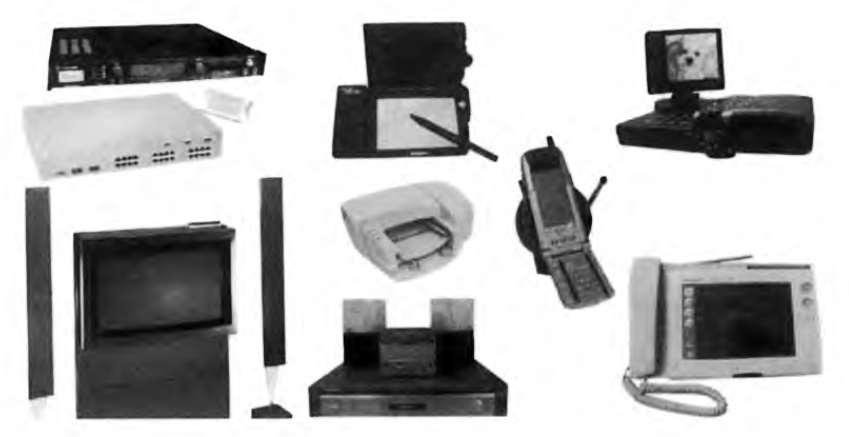
\includegraphics[width=0.8\textwidth]{Figuras/systems_embedded.PNG}
              \legend{Fonte: \cite{Li:2003:RCE:829584}}
            \end{figure}
    \par
    Uma definição geral para sistemas embarcados: são sistemas que realizam uma função dedicada e possuem a integração
    de hardware e software fortemente acoplados, geralmente são uma parte específica de um sistema maior \cite{Li:2003:RCE:829584}.
    
    \par
    % microcontroladores e microprocessadores
    Os microcontroladores e microprocessadores são dispositivos fundamentais nos sistemas embarcados, porém eles possuem algumas diferenças,
    entre as principais delas é que os microcontroladores já possuem todos os componentes necessários para seu funcionamento diferente dos microprocessadores que necessitam de outros componentes e periféricos para funcionar por exemplo memória, dispositivos de entrada/saída, conversores de sinais \cite{ayala:1991}.  
    
    \par
    Um exemplo de microcontrolador é o ATmega328P, que pode ser encontrado no Arduíno Nano, esse microcontrolador conta com 32 Kilobytes para a gravação de programas, 2 Kilobytes de SRAM (\textit{Static Random Access Memory}, Memória de acesso aleatório estático), 1 Kilobyte de EEPROM ( \textit{Electrically-Erasable Programmable Read-Only Memory}, Memória somente leitura programável apagável eletricamente) e 2 Kilobytes para o carregador de inicialização, ATmega328P pode ser visualizado na \autoref{fig:ATmega} \cite{arduino}.

   \begin{figure}[h!]
              \caption{\label{fig:ATmega}{Microcontrolador ATmega328P}}
              \centering
              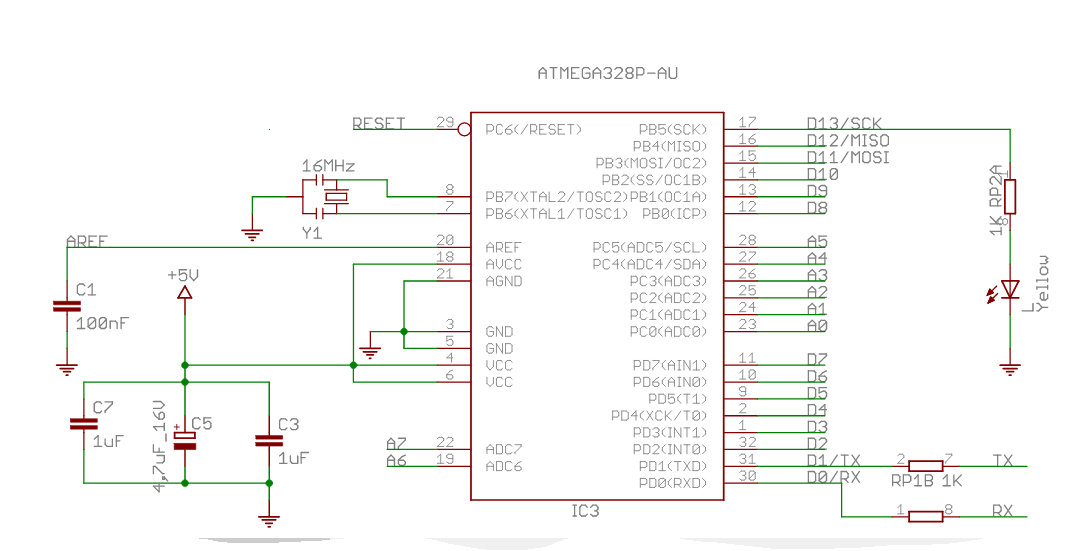
\includegraphics[width=0.3\textwidth]{Figuras/atmega.PNG}
              \legend{Fonte: \cite{arduino}}
    \end{figure}
 
    \par
    O Arduíno é uma popular ferramenta para desenvolvimento de aplicações IoT (\textit{Internet of things}, Internet das coisas), também sendo utilizado para ensino e seu hardware é \textit{Open Source} possibilitando que a comunidade contribua com tutoriais e suporte. O Arduíno Nano é mostrado na \autoref{fig:arduino nano}, é uma placa difundida e designers, engenheiros, estudantes, desenvolvedores e fabricantes de todo o mundo estão usando o Arduíno para inovar \cite{arduino}.
     \begin{figure}[h!]
              \caption{\label{fig:arduino nano}{Arduíno Nano}}
              \centering
              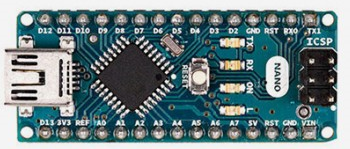
\includegraphics[width=0.6\textwidth]{Figuras/arduino_nano.png}
              \legend{Fonte: \cite{arduino}}
    \end{figure}
    \par
    Uma outra ferramenta de desenvolvimento é o NodeMcu, uma placa \textit{Open Source} que combina o chip ESP8266 (ESP-12E) com a pilha de protocolos TCP/IP integrada, essa combinação possibilita a conectividade com rede WiFi. O NodeMcu conta com um processador (Tensilica LX106) podendo atingir 160MHz, possui uma memória RAM de 20KB e memória flash de 4MB. A linha de programação pode ser realizada utilizando LUA ou a IDE do Arduíno \cite{nodemcu}.
    \par
     \begin{figure}[h!]
              \caption{\label{fig:arduino nano}{NodeMcu}}
              \centering
              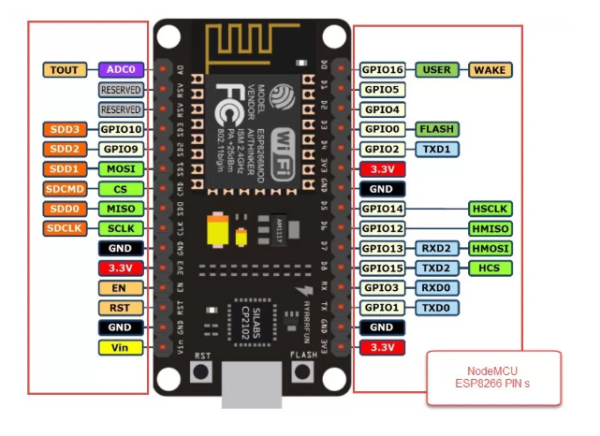
\includegraphics[width=0.6\textwidth]{Figuras/esp8266-nodemcu.png}
              \legend{Fonte: \cite{imgnodemcu}}
    \end{figure}
    \subsection{\textit{Internet of Things }(IoT)}
    \par
    A possibilidade de comunicação entre objetos de uso cotidiano do ambiente real com a internet referência o termo IoT, quando um objeto está conectado a rede de computadores e passa a transmitir informações de seu funcionamento ou estado, tal objeto passa a ser denominado de objeto inteligente \cite{iot2016}.
    \par
        % Esse balão "corrigir" não entendi muito bem o erro era so a forma da citação ou texto ?
    De acordo com \citeonline{iot2017}, o conceito de IoT não é novo, pois desde os passos iniciais da internet já se
    pensava em formas de traçar a comunicação entre objetos do dia a dia com a internet. Com os avanços de sistemas embarcados o
    desenvolvimento de uma infinidades de padrões e protocolos para a integração de
    WSN (\textit{Wireless sensor network}, rede de sensores sem fio) tornaram IoT uma realidade.
    \begin{figure}[H]
              \caption{\label{fig:iot}{Internet of Things.}}
              \centering
              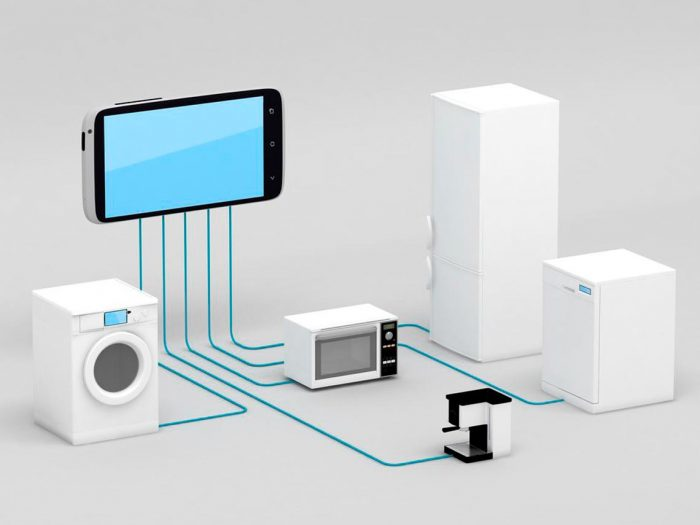
\includegraphics[width=0.5\textwidth]{Figuras/iot.png}
              \legend{Fonte: \cite{imgIot}}
        \end{figure}
    \par

    A \autoref{fig:iot} representa bem o cenário que IoT proporciona, na imagem é possível notar que todos os objetos estão conectados por
    uma espécie de cabo azul, mas isso é só uma representação, essa conexão também pode ser através de conectividade sem fio. Ainda
    sobre a imagem, o \textit{smartphone} tem um papel interessante, pois ele está sendo o encarregado de mostrar as informações enviadas
    pelos objetos para o usuário.

    \citeonline{homesmart} em seu trabalho, propõem um sistema \textit{smart home} que contém os serviços de automação residencial controle de ar-condicionados, umidificadores, filtros de ar e movimentos das cortinas baseados nas informações do clima, segurança doméstica para prevenir explosões e acidentes e o último serviço é o gerenciamento através da internet é um exemplo real de que os conceitos de IoT vem sendo estudados e implementados no dia-a-dia. Muitas aplicações vêm sendo desenvolvidas para o conforto, segurança ou monitoramento partindo dos conceitos de IoT.
    
\section{Comunicação Sem Fio}
    \par
    A medida que os elétrons se movimentam ondas eletromagnéticas são criada no espaço, essas ondas são medidas de acordo com suas oscilações e chamadas de frequência (Hertz), o comprimento dessa onda é medido pela distância de dois pontos máximos ou dois pontos mínimos seguidos \cite{tenenbaum2002}.
    %\par
    Segundo \citeonline{tenenbaum2002} ao colocar uma antena em um circuito elétrico apropriado pode-se  transmitir e receber ondas
    eletromagnéticas, a comunicação sem fio é baseada nisso.
    
    \subsection{Transmissão por rádio}
        % o que é
        
        \par
        A transmissão de dados por rádio pode acontecer de duas maneiras: não-direcional e direcional  \cite{torres2001}.
        
        \begin{itemize}
        \item{Não-Direcional: }
        Quando a transmissão é feita pela forma não-direcional, a frequências são emitidas em todas as direções e qualquer antena localizada na região de alcance das ondas de rádio podem captar os dados \cite{torres2001}, isso pode ser visto na \autoref{fig:nao_direciona}.
            \begin{figure}[H]
              \caption{\label{fig:nao_direciona}{Transmissão não-direcional.}}
              \centering
              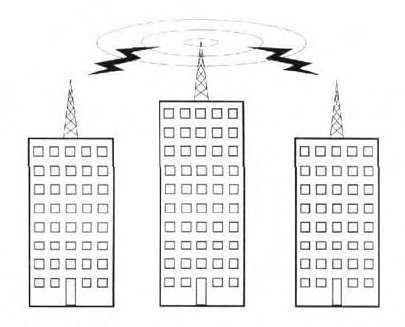
\includegraphics[width=0.3\textwidth]{Figuras/transmissao_radio_nao_direcional.PNG}
              \legend{Fonte: \cite{torres2001}}
            \end{figure}
        \par
        A  \autoref{fig:nao_direciona} mostra que as ondas de rádio são emitidas em todas as direções e que qualquer antena/receptor que estiver no alcance pode receber os dados do emissor.
        
        \item{Direcional: }
        A transmissão no sistema direcional necessita que os aparelhos transmissores e receptores estejam apontando um na direção do outro para que haja comunicação, sem contar que não pode ter obstáculos entre eles senão dificulta a transmissão \cite{torres2001}. A \autoref{fig:direcional} exemplifica o funcionamento dessa forma de transmissão.

        \begin{figure}[H]
              \caption{\label{fig:direcional}{Transmissão direcional.}}
              \centering
              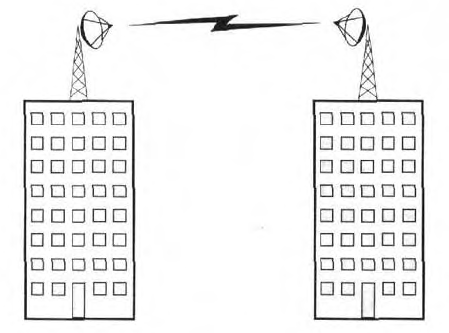
\includegraphics[width=0.3\textwidth]{Figuras/transmissao_radio_direcional.PNG}
              \legend{Fonte: \cite{torres2001}}
        \end{figure}
        \par
        De outro modo a \autoref{fig:direcional} mostra que o primeiro transmissor deve estar direcionado para a direção do segundo transmissor, e assim deve acontecer com o segundo transmissor também.
        \end{itemize}    
\section{Localização}
\par
Segundo \citeonline{rfid2009review}, as informações situacionais de pessoas ou objetos têm um papel muito importante nas aplicações, dessa forma é possível saber a posição dos objetos ou pessoas para assim fazer um monitoramento ou utilizar para várias outras aplicações. Essas informações podem ser obtida através de sistemas de posicionamento, que podem ser classificados dependendo do ambiente, podendo ser destinada a ambientes internos ou externo. Esta seção aborda alguns dos tipos de sistemas de localização.
    \subsection{GPS}
    \par
    GPS é um sistema de posicionamento global implementado pelo programa NAVSTAR \textit{(Navigation System Timing and Ranging)}, iniciado no ano de 1973. Era mantido pela divisão de sistema espacial dos Estados Unidos e era destinado apenas para uso militar \cite{gpsEduardo2005}.
    \par
   O principal objetivo do uso de GPS é determinar as coordenadas espaciais de pontos referentes a um sistema mundial, para isso o sistema faz uso de distâncias entre quatro satélites, a posição do receptor é calculada a partir dos sinais recebido pelos satélites \cite{gpsEduardo2005}.

   \begin{figure}[H]
              \caption{\label{fig:satelites}{Constelação de Satélites.}}
              \centering
              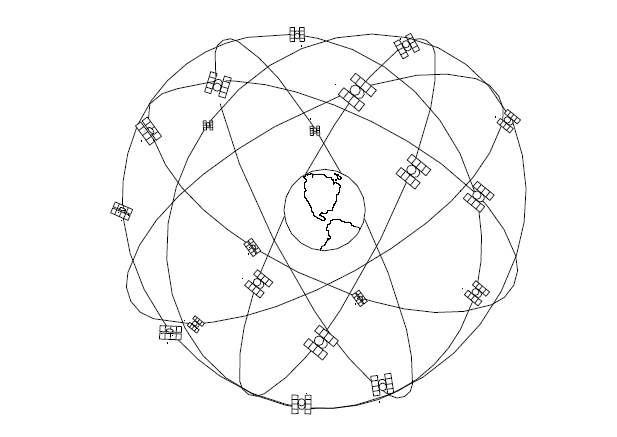
\includegraphics[width=0.5\textwidth]{Figuras/gps_satelites.PNG}
              \legend{Fonte: \cite{gpsEduardo2005}}
        \end{figure}
        \par
        A  \autoref{fig:satelites} mostra a movimentação dos satélites em torno da Terra para assim enviar sinais para os receptores que por sua vez interpretam esses sinais resultando em seu posicionamento na Terra.
 
    \subsection{WLAN\label{subsection:wlan}}
    \par
    A localização em ambientes indoor utilizando WLANs pode ser feita com a RSSI, \textit{Angle of Arrival} (AOA), ou \textit{Time Difference of Arrival} (TDOA) \cite{wifiFernandes}. Os dispositivos devem possuir conectividade sem fio para que seja possível saber seu posicionamento no ambiente. A função que permite a utilização de RSSI está disponível em todas as interfaces 802.11 \cite{Wlan2012}.
    
    \par
    Entre as inúmeras maneiras de localizar dispositivos em ambientes fechados utilizando WLANs, algumas são:
    \begin{itemize}
        \item {Triangulação:}
        \par
        Essa forma de localizar faz uso de AOA (\textit{angle of arrival}), que seria computação dos ângulos a múltiplos ponto de acesso, o resultado disso é uma interceptação que resulta na provável localização, isso pode ser visto na \autoref{fig:triangulacao} \cite{wifiFernandes}.
           \begin{figure}[H]
              \caption{\label{fig:triangulacao}{Triangulação.}}
              \centering
              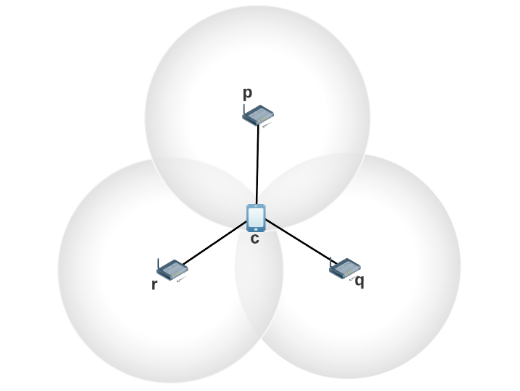
\includegraphics[width=0.5\textwidth]{Figuras/triangulacao.PNG}
              \legend{Fonte: \cite{wifiFernandes}}
        \end{figure}
        \item {Trilateração: }
        \par
       Utilizando propriedades geométricas essa técnica faz cálculos entre múltiplos pontos de acesso para assim obter a posição do dispositivo \cite{wifiFernandes}.
        \begin{figure}[H]
              \caption{\label{fig:trilateracao}{Trilateração.}}
              \centering
              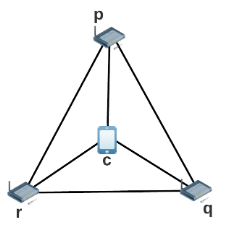
\includegraphics[width=0.3\textwidth]{Figuras/trilateracao.PNG}
              \legend{Fonte: \cite{wifiFernandes}}
        \end{figure}
       \par
        Na \autoref{fig:trilateracao} é mostrado que há uma a comunicação entre os pontos de acesso para assim poder efetuar os cálculos, esses cálculos são uma forma de saber a TDOA (\textit{time difference of arrival})  para assim estimar a posição do objeto \cite{wifiFernandes}.
        
        \item {Reconhecimento de padrões:}
        \par
        O RSS (\textit{received strength signal}) é o principal requisito dessa técnica, em que é feita medições prévias para fazer uma comparação com os dados do banco de dados. Inicialmente é necessário uma fase em que é feita a calibração para se obter o mapa de assinatura \cite{wifiFernandes}.
        
        \par
        O mapa de assinatura é basicamente dados do banco que representam a coleção das medidas de RSSI (\textit{received strength signal indicator}) em diferentes locais para todos os pontos de acesso no ambiente \cite{wifiFernandes}. Na \autoref{fig:fingerprinting} é mostrado seu funcionamento, onde cada ponto de acesso se comunica com o servidor para assim fazer uma comparação com os dados do mapa de assinatura.
         \begin{figure}[H]
              \caption{\label{fig:fingerprinting}{Reconhecimento de padrões.}}
              \centering
              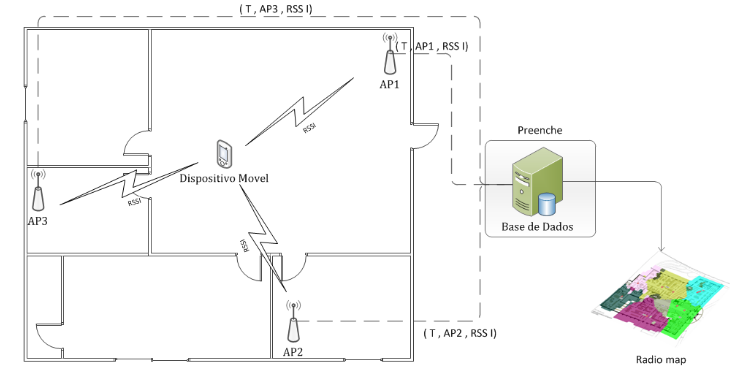
\includegraphics[width=0.7\textwidth]{Figuras/fingerprinting.PNG}
              \legend{Fonte: \cite{wifiFernandes}}
        \end{figure}
    \end{itemize}

    \subsection{RFID}
    \par
    Nessa subseção estaremos mostrando a técnica de localização com RFID utilizada no sistema \textit{LocAlizatioD iDentification based on dynaMic Active Rfid Calibration} (LANDMARC) proposto por \citeonline{landmarc}, visto que esse sistema é citado na grande maioria das fontes que retratam a utilização de RFID para localizar objetos em ambientes fechados.
    
    \par
    O LANDMARC faz uso de tags RFID ativas para determinar o local das tags que serão localizadas, essas tags ativas são colocadas em pontos já conhecidos pelo sistema e servem como pontos de referência e assim diminuir o número de leitores e ter uma melhor precisão no ambiente \cite{RFIDapplicationsTechniques}.
    
    \par
    Através das tags ativas é possível se obter informações com relação a intensidade do sinal, essa informação é utilizada para calibrar a distância para as tags de rastreio por meio de uma soma com o peso atribuído às tags de referências mais próximas, é importante ressaltar que a precisão dos resultados depende da forma que as tags de referência são posicionadas \cite{RFIDapplicationsTechniques}.
    
    \begin{figure}[H]
              \caption{\label{fig:landmarc2a}{LANDMARC.}}
              \centering
              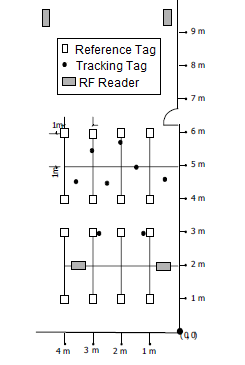
\includegraphics[width=0.4\textwidth]{Figuras/landmarc2a(1).png}
              \legend{Fonte: \cite{landmarc}}
        \end{figure}
    \par
    Na \autoref{fig:landmarc2a} mostra a aplicação sendo utilizada em um ambiente real por \citeonline{landmarc}, em que os retângulos cinzas são leitores RFID, os retângulos brancos são tags de referências e os pontos pretos são tags a serem localizadas, e dessa forma o sistema calcula as coordenadas dos objetos.
\begin{comment}    
    \subsection{Sistemas de Localização }
     \begin{itemize}
        \item{LANDMARC}
        \item{RADAR}
        \item{SpotON}
     \end{itemize}
\end{comment}    
\section{Algoritmos de Localização indoor}
Nesta seção serão abordados alguns dos algoritmos que já foram utilizados para localização em ambientes indoor.
    \subsection{Multilateração}
    A multilateração estima a coordenadas do nó de destino a partir das distâncias do nó de destino para o nó de referência que possui coordenadas conhecidas, é o mesmo que ocorre na trilateração, porém a multilateração pode-se utilizar 2,3 ou n nós de referências, é um método utilizado para suprir a trilateração. A inserção de mais nós tem por finalidade aumentar a precisão e diminuir a região de incerteza \cite{rfid2009review}.
    \par
    Segundo \citeonline{rfid2009review} os cálculos são executados da seguinte forma, havendo \textit{n} nós de referência, que serão
    representado por $R_k$,  $k = \left[ 1, 2, ... , n \right] $ com suas coordenadas já conhecidas $( x_k, y_k )$, $T$ representando
    o nó alvo com coordenadas desconhecidas $(x,y)$, podemos estimar utilizando a fórmula da distância da geometria analítica:
    
    \begin{equation}
    \left \{ \begin{array}{c}
        r_1^2 = (x - x_1 )^2 + (y - y_1)^2  \\
        r_2^2 = (x - x_2 )^2 + (y - y_2)^2  \\
        ...  \\
        r_n^2 = (x - x_n )^2 + (y - y_n)^2
   \end{array} \right.
    \end{equation}

    \par
    Depois subtraímos cada uma das equações a partir da primeira para
    denotar $b_{i1}= \frac{1}{2}(x_1^2 - x_i^2 + y_1^2 -y_i^2 + r_i^2 - r_1^2)$, sendo que $i = [2,3, ..., n]$ e em seguida
    linearizar o sistema (Equação~\ref{eq:lin})
     que também pode ser escrito no formato de matriz $b = AX$. Esse algoritmo requer pouca computação e está em uso em muitos sistemas de localização.    

    
    \begin{equation}
    \left \{  \begin{array}{c}
        b_{21} = x(x_1 - x_2) + y(y_1 - y_2)  \\
        b_{31} = x(x_1 - x_3) + y(y_1 - y_3)  \\
        ...  \\
        b_{n1} = x(x_1 - x_n) + y(y_1 - y_n)
   \end{array} \right.
        \label{eq:lin}
    \end{equation}


    \subsection{Inferência Bayesiana}
  Segundo \citeonline{bayesian2001} a inferência bayesiana é dedução estatística através de evidências ou análise observatória para que a inferência de uma hipótese possa vir a ser verdadeira, e no caso da localização de um dispositivo isso pode ser realizado utilizando RSS entre o nó de destino e os pontos de acesso.


    \begin{figure}[H]
              \caption{\label{fig:bayesian}{Rede Bayesiana}}
              \centering
              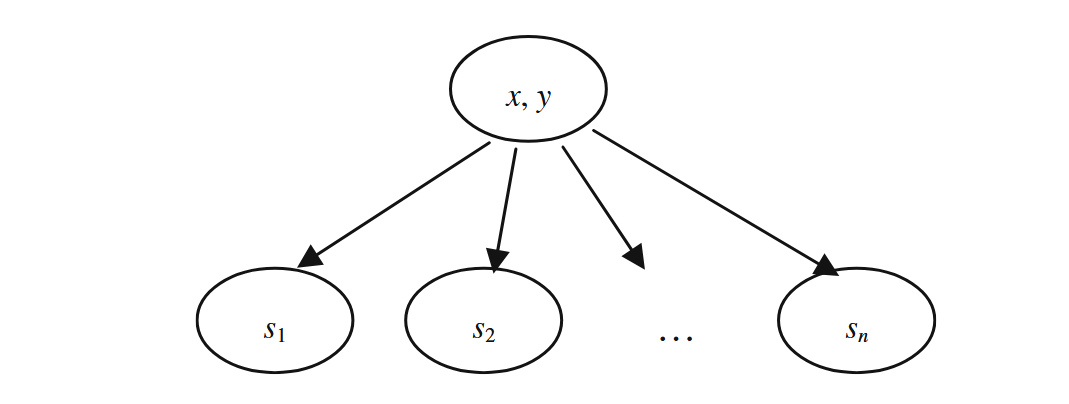
\includegraphics[width=0.7\textwidth]{Figuras/bayesian_network.PNG}
              \legend{Fonte: \cite{rfid2009review}}
        \end{figure}

        Na \autoref{fig:bayesian} temos uma representação de uma rede bayesiana para localização estacionária, onde as coordenadas $(x,y)$ representam o nó que será localizado e o $S_i$, $i=1,...,n$ são uma série de intensidades de sinais transmitidas ou recebidas pelos pontos de referências do sistema, como nesse sistema as probabilidade de $S_i$ são independentes e não interferem uma na outra dizemos que há uma satisfação em relação a condição de Markov \cite{rfid2009review}.
        \par
        \citeonline{rfid2009review} afirma que a localização do dispositivo alvo pode ser obtida através da fórmula recursiva
        $P((x,y) | s_1, s_2, ..., s_n) = \alpha P(s_n | (x,y)) \times P((x,y) | s_1,s_2, ...,s_{n-1})$, nesta expressão $\alpha$ é um fator de normalização para que a soma da probabilidade posterior, no caso a primeira parte da expressão $P((x,y) | s_1, s_2, ..., s_n)$ seja uma e $(s_n | (x,y))$ calcule a probabilidade da RSSI dada para a localização do dispositivo, é importante ressaltar que essa é uma expressão para localizar alvos estáticos.
        
    \subsection{K-Nearest-Neighbor}
    Os algoritmos de vizinhança ou no caso de \textit{nearest-neighbor} tem uma abordagem bem simples que envolve
    utilizar os nó já classificados para classificar os novos nós a partir da medida de similaridade \cite{knn-3dLAN},
    de outro modo, utilizar-se dos seus vizinhos para assim obter suas coordenadas com os cálculos baseados em RSS \cite{rfid2009review}.
    %
    Algumas das métricas abordada por \citeonline{knn-3dLAN} são:

    \begin{itemize}
    \item Distância Euclidiana
      \par
      $Dist(r,s) =  \sqrt{(x_r - x_s)(x_r - x_s)^\prime}$
    \item Padronização da Distância Euclidiana
      \par
      $Dist(r,s) =  \sqrt{(x_r - x_s)D^-1(x_r - x_s)^\prime}$
    \item Distância de Mahalanobis
      \par
        $Dist(r,s) =  \sqrt{(x_r - x_s)V^-1(x_r - x_s)^\prime}$
    \item Distância de Manhattan
      \par
      $Dist(r,s) = \sum_{j=1}^{n} |x_{rj} - x_{sj}|$
    \item Distancia de Minkowski
      \par
      $Dist(r,s) = \sqrt[p]{\sum_{j=1}^{n}|x_{rj} - x_{sj}|^p}$

    \end{itemize}
   \par
   \citeonline{rfid2009review} faz mostra uma outra abordagem para calcular as coordenadas do alvo obtidos a partir do sistema a seguir:
   
   \begin{equation}
   \left \{ \begin{array}{c}
        x= \sum_{i=1}^{k}w_{i}x_{i}   \\
        y= \sum_{i=1}^{k}w_{i}y_{i}  
   \end{array} \right.
   \end{equation}
    
    Nesse sistema o $k$ representa a quantidade de vizinhos, $(x_i,y_i)$ são as coordenadas dos pontos de referências vizinhos e $w_i$ os pesos desses pontos, o cálculo dos pesos é feito a partir da diferença de RSSI entre os pontos de referências e o alvo e as fórmulas para tal são:
    \begin{itemize}
        \item $w_i = \frac{1 / \sum_{j=1}^{m}|s_{ij} - s_{j}|}{\sum_{j=1}^{k} (1/ \sum_{j=1}^{m}|s_{ij} - s_{j}|)}$
        
        \item  $w_i = \frac{1 / \sqrt{\sum_{j=1}^{m}(s_{ij} - s_{j})^2}}{\sum_{j=1}^{k} (1/ \sqrt{\sum_{j=1}^{m}(s_{ij} - s_{j})^2})}$
    \end{itemize}$\\$
    nas expressões de $w_i$, dizemos que $s_j$ e $s_{ij}$, $j =1, ..., m$ representam  RSSI dos respectivos ponto de referências e nó alvo que será localizado.
    
    \subsection{Proximidade}
    A técnica de Proximidade, segundo \citeonline{rfidProximity} baseia-se no princípio de que se o alvo está no alcance de uma antena ou leitor, sua localização será a mesma que a da antena e se o alvo está no alcance de duas ou mais antenas, a localização dada é aquela cujo possui a intensidade do sinal mais forte. Já para \citeonline{rfid2009review} quando o alvo está no alcance de dois ou mais receptores, utiliza-se o cálculo de centroide para estimar a localização.
    
\section{Node.js}
    De acordo com \citeonline{node} Node.js é um ambiente para desenvolvimento \textit{server-side} que utiliza JavaScript como linguagem de programação. É baseado no V8 um interpretador JavaScript desenvolvido pela Google e ambos são implementados em C e C++ para ter baixo consumo de memória e alta performa, isso só é possível pois antes de executar, o código é compilado para linguagem nativa para em seguida ser executado.
    \par
    Node.js é uma plataforma escalável permitindo a programação direta com os protocolos de rede ou a utilização de bibliotecas para acessar os recursos do sistema operacional. Uma outra vantagem do Node.js é que ele possui seu próprio gerenciado de pacotes o NPM (\textit{Node Package Manager}), através dele é possível instalar, remover, listar ou atualizar novos módulos \cite{pereira2014aplicacoes}.
    \par
    Alguns módulos do Node.js:
    \begin{itemize}
        \item Mongoose: é uma biblioteca que tem como finalidade a modelagem de objetos do MongoDB;   
        \item Express: é uma biblioteca que fornece ferramentas e recursos para desenvolver aplicações web e sistema de roteamento;
        \item Body-parser: é um analisador de requisição sob a entrada \textit{req.bory};
        \item EJS: é uma linguagem de \textit{templates} quer permite gerar marcações HTML com JavaScript;
        \item Moment: é uma biblioteca para manipulação, validação, analisa e formatar datas;
        \item Fs: é uma biblioteca para manipulação e criação de arquivos;
        \item Nodemailer: é uma biblioteca para envio de e-mail a partir da aplicação.
    \end{itemize}
\section{MongoDB} 
    Segundo \cite{mongodb} o MongoDB é um sistema de gestão de base de dados(SGBD) NoSQL (não relacional), \textit{open source} e multiplataforma. Foi desenvolvido utilizando a linguagem de programação C++ em 2007. O MongoDB utiliza o formato BSON (Binary JSON) para armazenar os documentos, tais documentos são agrupados em coleções de acordo com sua estrutura e a identificação é feita por meio de ID, também podendo ser feita de maneira combinatória com ID e \textit{timestamp}. 
    \par
    MongoDB é um SGBD ágil e muito escalável, o seu nome vem da palavra ``hu\textbf{mongo}us'' que enfatiza a escalabilidade e alto desempenho que o MongoDB fornece. Como é baseado NoSQL descarta o uso de colunas e linhas como em banco de dados relacional e basicamente faz uso de objetos como modelo \cite{dayley2014node}.
\section{Modelagem de Sistemas}
    Esta seção tem por finalidade apresentar as forma cujo os sistemas computacionais são modelados de maneira abstrata, o processo de modelagem de sistema tem papel importante pois ajuda a entender e extrair os requisitos necessários para a construção do sistema.
    \subsection{UML - \textit{Unified Modeling Language}}
    O UML (em português Linguagem de Modelagem Unificada) é uma linguagem cujo principal papel é a construção, visualização e documentação de projetos de sistemas. Surgiu na década de 90, tendo em vista que havia a necessidade de uma linguagem para modelagem que funcionasse como uma norma e fosse aceita e utilizada pela indústria, ambientes acadêmicos e de investigação \cite{uml}.
    \par
    Na UML é possível agrupar elementos e relacioná-los de maneira lógica ou estrutural, isso é o conceito de diagramas. Os elementos têm um papel importante nos modelos, eles estarão organizados de acordos com a função desempenhada no sistema, podendo representar componentes do sistema, usuário, interfaces \cite{uml}.
    
    \begin{figure}[H]
              \caption{\label{fig:uml-elementos}{Elementos UML}}
              \centering
              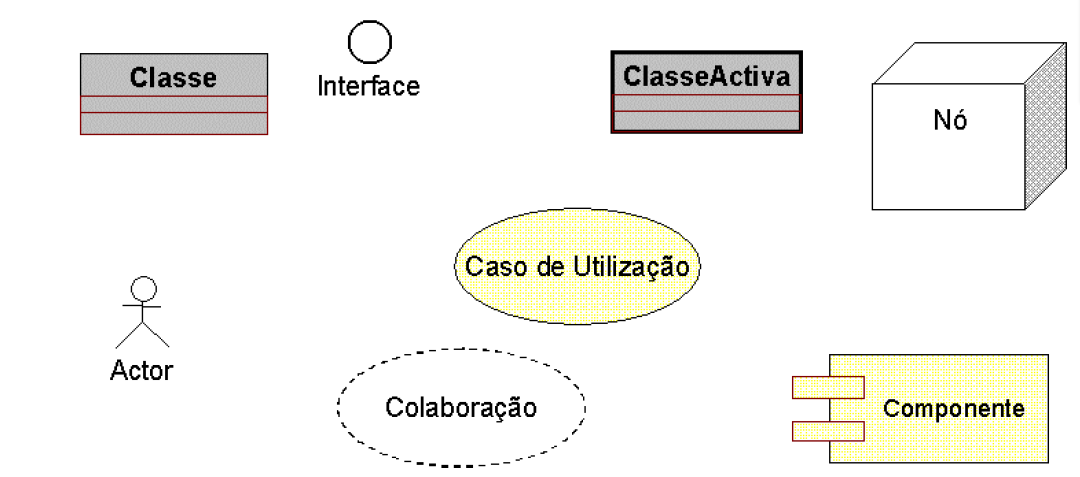
\includegraphics[width=0.9\textwidth]{Figuras/uml1.PNG}
              \legend{Fonte: \cite{uml}}
        \end{figure}
    \par
    Na \autoref{fig:uml-elementos} está um resumo de alguns elementos básicos que é utilizados em modelos de projetos de software, esses componentes por mais que sejam básicos, possibilitam a representação de vários componentes em um projeto. A seguir uma breve descrição dos diagramas comuns da UML.
    
    \begin{itemize}
        \item \textbf{Diagrama de Caso de Uso -}
        Descreve as funcionalidades do sistema, ou seja nesse diagrama é apresentado o que o sistema deve fazer e os serviços que serão disponibilizados para os utilizadores \cite{nunesfundamental}. 
    \end{itemize}
\begin{comment}
    

    \begin{itemize}
       \item \textbf{Diagrama de Classe -}
       Descreve a estrutura do sistema, como o modelo geral de informações utilizando orientação a objetos \cite{nunesfundamental}.
        
        \item \textbf{Diagrama de Caso de Uso -}
        Descreve as funcionalidades do sistema, ou seja nesse diagrama é apresentado o'que o sistema deve fazer e os serviços que serão disponibilizados para os utilizadores \cite{nunesfundamental}.
        
        \item \textbf{Diagrama de Estados -}
        Descreve o comportamento dos objetos, as representação dos possíveis estados de um objeto e eventos que alteram valores de atributos dos objetos desencadeando as transições \cite{uml}.
        
        \item \textbf{Diagrama de Sequência -}
        Descreve as interações dos objetos no sistema em determinado período de tempo. Essa interação é realizada por meio de troca de mensagens síncrona ou assíncrona e cada objeto possui uma linha temporal \cite{uml}.
        
        \item \textbf{Diagrama de Componentes -}
        Descreve interações entre objetos dando ênfase maior as ligações entre objetos e numerando as mensagens dessa forma não apresenta o tempo como no diagrama de sequência \cite{uml}.
        
        \item \textbf{Diagrama de Caso de Uso -}
        Descreve as funcionalidades do sistema, ou seja nesse diagrama é apresentado o que o sistema deve fazer e os serviços que serão disponibilizados para os utilizadores \cite{nunesfundamental}.
        
        \item \textbf{Diagrama de Estados -}
        Descreve o comportamento dos objetos, as representação dos possíveis estados de um objeto e eventos que alteram valores de atributos dos objetos desencadeando as transições \cite{uml}.
        
        \item \textbf{Diagrama de Atividade -}
        Descreve o fluxo de trabalho que classifica os estados de "estados de atividades", onde e realizados a transições quando há a conclusão das atividades dos estados anteriores \cite{uml}.
        
        \item \textbf{Diagrama de Sequência -}
        Descreve as interações dos objetos no sistema em determinado período de tempo. Essa interação é realizada por meio de troca de mensagens síncrona ou assíncrona e cada objeto possui uma linha temporal \cite{uml}.
        
        \item \textbf{Diagrama de Componentes -}
        Descreve interações entre objetos dando ênfase maior as ligações entre objetos e numerando as mensagens dessa forma não apresenta o tempo como no diagrama de sequência \cite{uml}.

    \end{itemize}

    \subsection{Redes de Petri}
        Redes de Petri é uma técnica utilizada para modelagem formal de sistemas que possuem atividade paralelas, concorrentes, assíncronas e não-determinísticas, também definida como modelo matemático para representação gráfica, esse modelo foi proposto por Carl Petri\cite{cardoso1997redes}. As redes de petri compõe-se de conjuntos de lugares, transições e tokens, os tokens são como fichas no modelo podendo ser produzidos ou consumidos nas transições,  \cite{formalVerificationUML}.
        
        \par
        De maneira formal \citeonline{formalVerificationUML} define rede de Petri como uma quintuplica $\langle P,T,F,W,u\rangle$, onde $P$ representa o conjunto finitos de lugares $\{ p_1, p_2,..., p_n \}$, $T$ representa o conjunto finito de transições $\{t_1, t_2,..., t_n\}$, $F$ representa o conjunto finitos de arcos $F\subseteq (P \times T) \cup (T \times P)$, $W$ é a relação de pesos associadas aos arcos $W : F \rightarrow \mathbb{N}$ , e por fim $u$ define a quantidade de tokens em cada lugar $u : P \rightarrow \mathbb{N}$.
        
        \par
        De acordo com \citeonline{cardoso1997redes} os elementos básicos da rede de Petri são:
        \begin{itemize}
            \item Lugar: indicam uma condição, estado parcial, procedimento, conjunto de recursos ou tempo de espera e são representados por um círculo;
            \item Transição: indica um evento que ocorre no sistema, é representado por uma barra ou retângulo;
            \item Token: são informações sobre o estado do lugar em um determinado tempo, é representado por um ponto no lugar.
        \end{itemize} Na \autoref{fig:rede_petri} é mostrado um exemplo onde podemos visualizar os elementos para uma representação de  uma rede de petri contendo lugares, transições e tokens.
        \begin{figure}[H]
              \caption{\label{fig:rede_petri}{Exemplo de rede de Petri}}
              \centering
              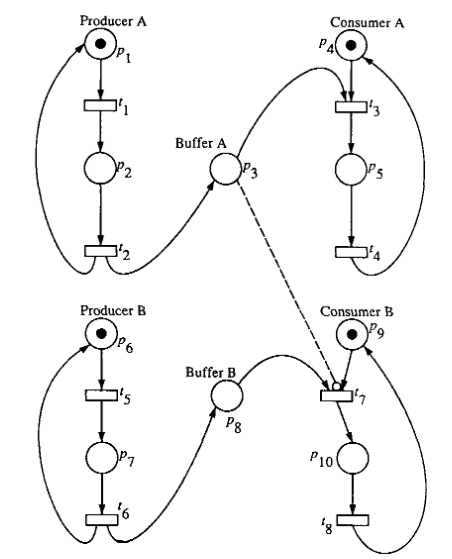
\includegraphics[width=0.7\textwidth]{Figuras/exemplo_rede_petri.png}
              \legend{Fonte: \cite{murata}}
        \end{figure}
        \par
        No exemplo da \autoref{fig:rede_petri} temos a representação de um sistema produtor-consumidor, onde o consumidor A tem prioridade sobre o consumidor B nesse sentido é possível notar que A pode consumir desde o \textit{buffer} A tenha tokens, contudo B só poderá consumir se o \textit{buffer} A estiver vazio e o \textit{buffer} B possuir tokens \cite{murata}.
\end{comment}

